\documentclass[11pt]{article}
\usepackage{fullpage}
\usepackage{setspace}
% load matlab package with ``framed'' and ``numbered'' option.
%\usepackage[framed,numbered,autolinebreaks,useliterate]{mcode}
\usepackage{listings}
\lstset{
	breakatwhitespace=true,
	breaklines=true,
	frame=single,
	keepspaces=true,
	numbers=left,
	numbersep=5pt,
	stepnumber=5,
	tabsize=3,
	language=MATLAB,
	basicstyle=\small
}
\usepackage{subfigure}
\usepackage{wrapfig}
\usepackage{graphicx}
\usepackage{cite}
%\usepackage{natbib}
\usepackage{booktabs}
\usepackage{fancyhdr}
\usepackage{amsmath}
\usepackage{amsfonts}
\usepackage{amssymb,amsmath,amsthm}
\usepackage{bm}
\usepackage[english]{babel}
\usepackage{multirow}
\usepackage{caption}
\usepackage{enumitem}
\usepackage{placeins}
\usepackage{adjustbox}
\usepackage[title]{appendix}
\newcommand{\vb}{\boldsymbol}
\newcommand{\vbh}[1]{\hat{\boldsymbol{#1}}}
\newcommand{\vbb}[1]{\bar{\boldsymbol{#1}}}
\newcommand{\vbt}[1]{\tilde{\boldsymbol{#1}}}
\newcommand{\vbs}[1]{{\boldsymbol{#1}}^*}
\newcommand{\vbd}[1]{\dot{{\boldsymbol{#1}}}}
\newcommand{\by}{\times}
\newcommand{\tr}{{\rm tr}}
\newcommand{\sfrac}[2]{\textstyle \frac{#1}{#2}}
\newcommand{\ba}{\begin{array}}
\newcommand{\ea}{\end{array}}
\newcommand{\sinc}{{\rm sinc}}
\renewcommand{\equiv}{\triangleq}
\newcommand{\cnr}{C/N_0}
\newcommand{\sgn}{\rm sgn}
\renewcommand{\Re}{\mathbb{R}}
\renewcommand{\Im}{\mathbb{I}}
\newcommand{\E}[1]{\mathbb{E}\left[ #1 \right]}


\title{ASE 372N \\ \huge \bfseries Extended Global Positioning System}
\author{\Large Matthew Cullen \textsc{Self}}
\date{\today}

%\title{\large ASE 372N \\ \Huge \bfseries Extended Global Positioning System}
%\author{\Large Matthew Cullen \textsc{Self}}
%\date{\vfill \hrule \vspace{1em} December 9, 2016 \pagebreak}

\begin{document}
%\onehalfspace
\maketitle
\hrule
\begin{abstract}
The feasibility of using GPS signals at altitudes high above the constellation has been evaluated. A model was synthesized and evaluated to produce carrier-to-noise ratios of observations at various places in orbit around Earth, and at various times. It has been found that, given modern tracking and acquisition systems, a receiver in High Earth Orbit will be able to determine their location based solely off of GPS signals if the geometry is favorable (more likely than not). The impact of antenna and receiver design on the observability of a position has been discussed (more gain results in a higher likelihood of observability). Antenna gain patterns have been observed in carrier-to-noise maps, validating the implemented models. Confirmation of prior experiments further indicates the model is correct. 
\end{abstract}


\section{Introduction}
Global Navigation Satellite System (GNSS) receivers work by very carefully beaming information from known locations to an unknown location and evaluating the resulting shifts and delays in the signals as they arrive. This commonly takes place as a mobile devices discover their locations in reference to the known positions of the GPS satellites. Usually these devices are at or near, the surface of the Earth - the use case for which GPS has been designed - thus GPS Satellite Vehicles (SVs) direct their information carrying signals towards the Earth. These signals are emitted by complex antenna systems, but the net result is effectively a hemisphere of radiation around the pointing direction (towards the center of the Earth). Because the GPS SVs are high in space ($\approx 20,200$ km altitude), the radiated signal does not fall only on Earth; some of the signal misses the Earth and is broadcast into an area surrounding the Earth. This overlap in signal coverage, forms the basis of the Space Service Volume (SSV), a region in space where GPS signals are available. The basis of this report is to examine the extent of the SSV and the viability of using GNSS signals in this region.

\subsection{Motivation}
Traditional methods of locating satellites rely on sporadic radar measurements to form a position and velocity estimate for a given SV. As more and more satellites are launched, the availability of radar measurements continues to decline (unless a SV is very important). To combat this, many satellites now have a GNSS receiver to provide navigational solutions formed not from ground based observations, but instead formed continuously from GNSS signals. This trend has been accelerated by the increasing quality and availability of GNSS receivers, making GNSS tracking of satellites cheaper and more reliable.

Furthermore, it has been proven that GPS based navigation solutions are possible even from ``above the constellation,'' or at altitudes greater than the orbit of GPS satellites. Starting in 1990, a classified geosynchronous satellite ($\approx 36,000$ km altitude) used GPS signals at least in part of its navigation solution \cite{class}. The Radio Amateur Satellite Corporation (AMSAT) OSCAR-40 satellite was able to sporadically track satellites at an altitude of 59,000 km \cite{ao40}. NASA's Manetospheric Multi-Scale (MMS) mission, with a recently developed high gain receiver, was able to continuously track at least four satellites (the number required for a navigation solution) at altitudes of 70,000 km \cite{ssv}. These results form the baseline for additional studies into the feasibility of GPS navigation in High Earth Orbit.

\subsection{Theory}
The governing equations that determine whether or not a signal can be tracked or not are presented below in Equations \ref{eq:pow} and \ref{eq:cn0} (from \cite{ao40}).
\begin{equation}
\hat{P_r} = P_{out} + G_t + L_d + G_r
\label{eq:pow}
\end{equation}

\begin{equation}
\widehat{C/N_0} = \hat{P_r} + N_T + 228.6 + L_{sys}
\label{eq:cn0}
\end{equation}

The estimated received power, $\hat{P_r}$, is a function of the emitted power, $P_{out}$, the transmitter gain, $G_t$, the receiver gain, $G_r$, and the free space attenuation $L_d < 0$. The attenuation follows the inverse-square law such that the decibel reduction is equal to \[ 20\log(\frac{\lambda}{4\pi \rho}). \] Once the received power has been estimated, an estimate of the carrier to noise ratio ($\cnr$) can be formed based on the thermal noise, $N_T < 0$, and the system losses due to front end noise and conversion losses, $L_{sys} < 0$. The thermal noise can be modeled as \[ N_T = -10 \log(T_{sys})\] where $T_sys$ is the equivalent system noise temperature. The resulting $\cnr$ determines whether a satellite can be tracked. If the $\cnr$ is above a threshold particular to the receiver, then the signal is deemed ``observable.'' 

Many of the parameters are dependent on the receiver (e.g. receiver gain, system losses, thermal noise, and  $\cnr$ threshold). These values can be systematically determined, and are particular to the antenna being used, the receiver hardware and software, and other implementation details.

The parameter of interest for this report is the transmitter gain, $G_t$. Lockheed Martin has released the antenna gain patterns of many GPS satellites, making it possible to model the antenna gain accurately as a function of transmitter and receiver locations \cite{lockheed}. Crucially, the gain is dependent on two angles: the offbore angle, $\theta$, and the polar angle, $\varphi$. These two angles can be calculated based on the attitude of the transmitting satellite and the relative position vector. Then those angles can be used to determine the resulting directive gain of the transmission. Figure \ref{fig:examplegain} shows an example of the gain pattern. Inside low values of $\theta$, the gain is extremely high - this corresponds to the portion of the satellite's signal that is broadcast towards the Earth. There are additional ``sidelobes'' that extend outside this primary range, providing additional gain at some angles of $\varphi$.

\begin{figure}[h]
\centering
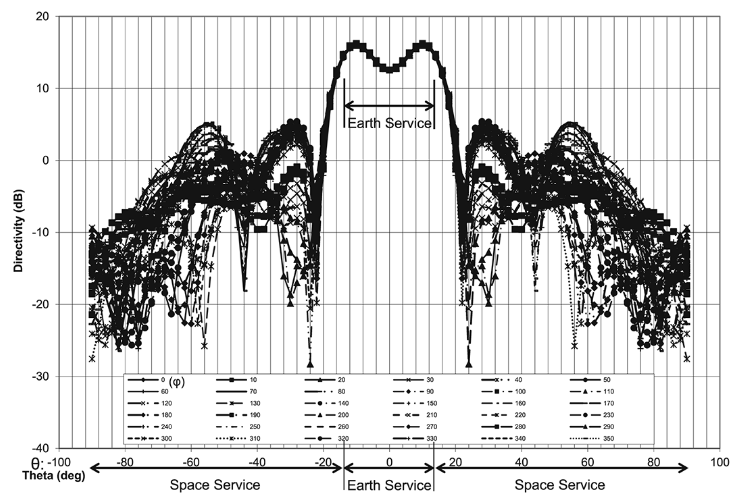
\includegraphics[width=.75\textwidth]{../Images/examplegain.png}
\caption{Typical L1 Gain Pattern}
\label{fig:examplegain}
\end{figure}

To calculate $\theta$ and $\varphi$, a yaw-steering attitude model was assumed \cite{orient}. This means that the satellite maintains a constant orientation towards the sun by varying a yaw angle around the primary pointing axis. This yaw angle, $\psi$ can be found in terms of the $\beta$ and $\mu$, the angles between the sun and the orbital plane and the satellite and midnight (see Fig. \ref{fig:geom}).
\begin{equation}
\psi = \text{atan2}(-\tan(\beta),\sin(\mu))
\label{eq:yaw}
\end{equation}

\begin{figure}[h]
\centering
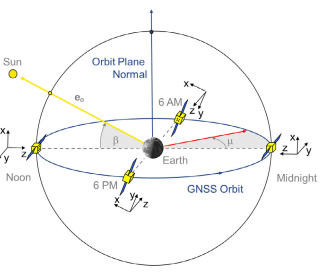
\includegraphics[width=.5\textwidth]{../Images/geom.png}
\caption{Sun - Earth - Satellite Geometry}
\label{fig:geom}
\end{figure}

This yaw angle, combined with a local orbital frame defined by the radial, along-track, and cross-track directions, makes it possible to relate the satellite position in ECEF to the Lockheed Martin prescribed body fixed axis. 

\FloatBarrier
\subsection{Implementation}
Taken together, the previous section describes a model for transmission and reception of a SV's signal. This was coded in MATLAB as a series of functions that can be called from a master script. Core to the process is the \verb|findRotationAngle| function, which takes a structure containing a satellite's position, velocity, the relative position vector, and the time, and returns $\varphi$ and $\theta$. This is completed by first finding the position of the Sun in the ECEF frame (nontrivial, relies on \verb|findSun| \cite{astro}), then relating that to the yaw angle, and finally using the yaw angle and position to find the directional cosine matrices necessary to find the body fixed axes in the ECEF frame.

A lookup function was implemented as \verb|SatDirectivityGain|, which takes $\varphi$ and $\theta$ as inputs, then performs the necessary bilinear interpolation. These were synthesized together in several experiments that tested the effects of various parameters on the number of tracked satellites.


\section{Results and Analysis}
\subsection{Single Satellite}
A single transmitting satellite was modeled. At a given instant in GPS time, the position of a satellite was determined, then the effects of changing several parameters were determined. The angles for $\phi$ and $\theta$ were calculated as a function of height above the North Pole, a region which was determined to have moderate visibility of the satellite. Figure \ref{fig:phiandtheta} shows the two plots. Note how the offbore angle $\theta$ is negative and drops below $-90\deg$. The drop below $-90\deg$ reflects that, at a certain altitude, the receiver is now behind the transmitter, and is unable to acquire any signals.

\begin{figure}[h]
\centering
\begin{minipage}{0.45\linewidth}
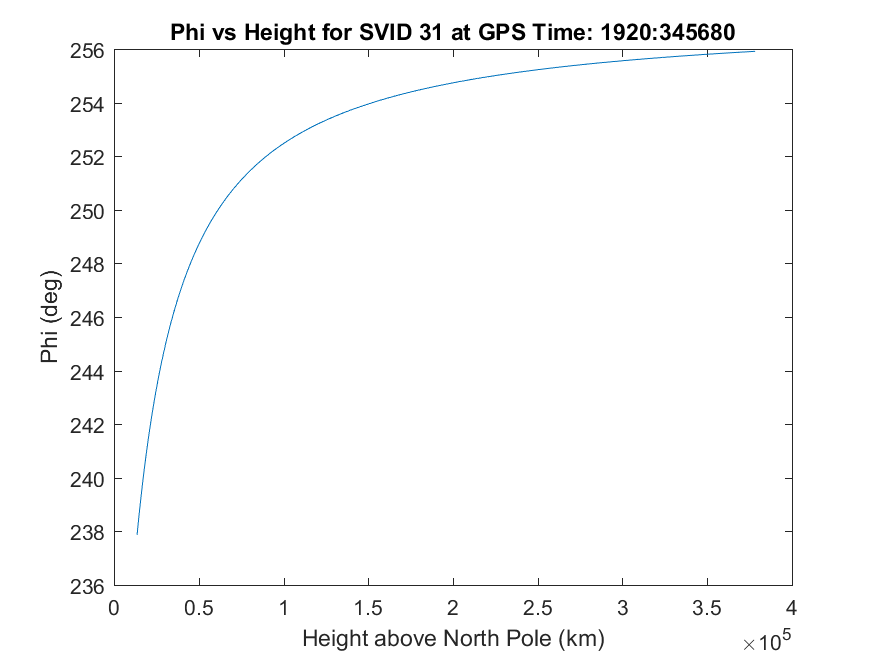
\includegraphics[width=\textwidth]{../images/phivsheight.png}
\caption{Phi}
\end{minipage}
\begin{minipage}{0.45\linewidth}
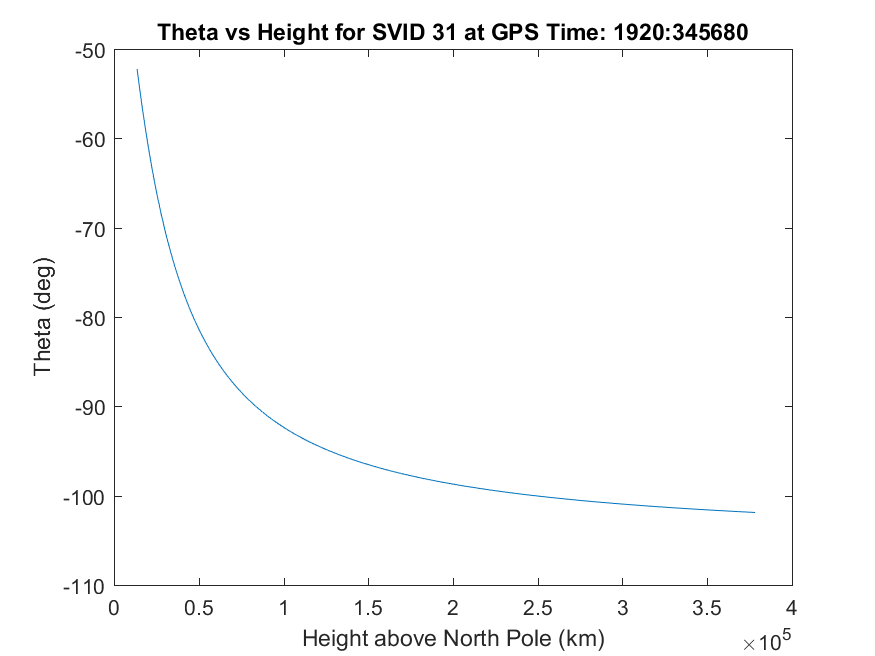
\includegraphics[width=\textwidth]{../images/thetavsheight.png}
\caption{Theta}
\end{minipage}
\caption{Angles vs Altitude}
\label{fig:phiandtheta}
\end{figure}

Figure \ref{fig:cnonorthpole} shows the modeled unbiased carrier to noise ratio. The unbiased carrier to noise ratio is found by setting the net gain and attenuation of the receiver and antenna to 0 dB, modeling a ``nuetral'' receiver. The biased, or actual received $\cnr$ can be found by adding back in the appropriate net gain to the unbiased $\cnr$. At precisely the same altitude that $\theta = 90\deg$, the $\cnr$ drops to 0, indicating that the signal isn't observable under any circumstances. The $\cnr$ plot also shows the presence of two side lobes extending beyond the main center lobe.

\begin{figure}[h]
\centering
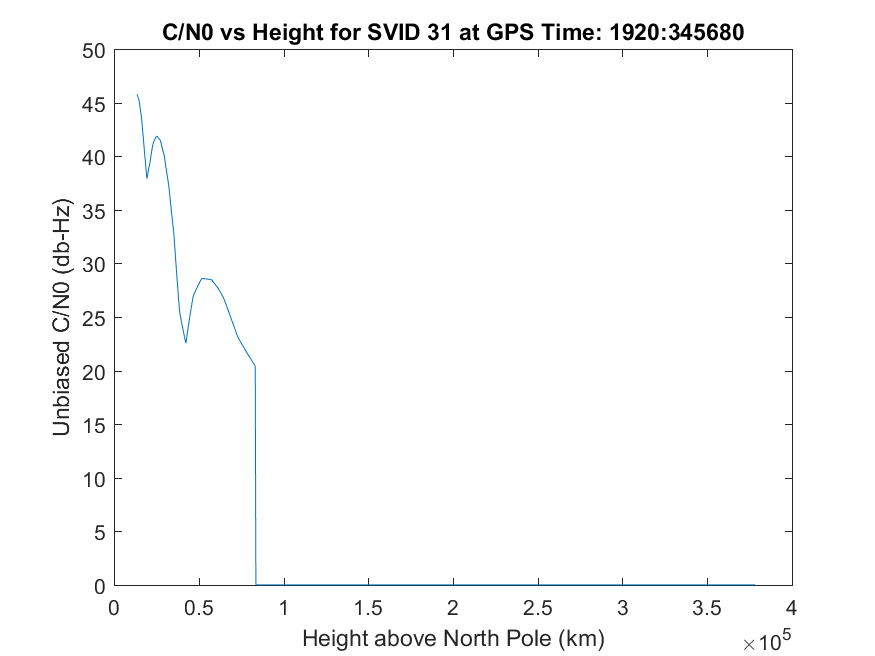
\includegraphics[width=.75\textwidth]{../Images/cn0vsheight.png}
\caption{$\cnr$ vs Altitude}
\label{fig:cnonorthpole}
\end{figure}

To better visualize the space in which a signal is observable, a mesh of locations was generated along the equatorial axis, extending to $\pm$100,000 km in both the ECEF x and ECEF y directions. The unbiased $\cnr$ was then plotted at each individual location, yielding Figure \ref{fig:cn0actual}. The plot has two main leaves, separated by the Earth's umbra, and bounded by the plane of the transmitting antenna. In each leaf, the side lobe gain patterns can be seen as certain lines of constant $\theta$ tend to have exceptionally high gains.

\begin{figure}[h]
\centering
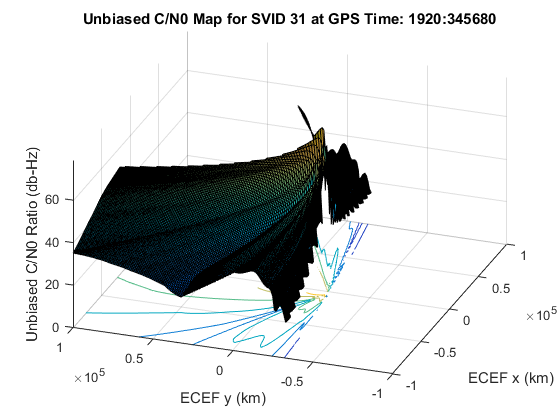
\includegraphics[width=.75\textwidth]{../Images/cn0mapactual.png}
\caption{$\cnr$ vs Position (Real Position)}
\label{fig:cn0actual}
\end{figure}

To get a idealized plot of the side lobes, the transmitting satellite was modeled as being on the ECEF x-axis instead of in its proper 3 dimensional space. This had the effect of constraining $\varphi$ and $\theta$ to varying along the x-y plane that the receiver is modeled in. Figure \ref{fig:cn0xaxis} shows clearly the antenna gain pattern in the contour map on the floor of the plot. The highest $\cnr$ is closest to the antenna boresight, right outside the Earth's shadow. In actual mission planning, care must be taken not to optimize $\cnr$ so much that the received sigal actually passes through the Earth's atmosphere.

\begin{figure}[h]
\centering
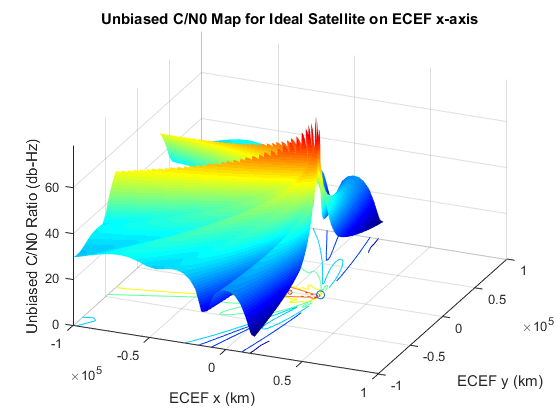
\includegraphics[width=.75\textwidth]{../Images/cn0mapxaxis.png}
\caption{$\cnr$ vs Position (Modeled Position)}
\label{fig:cn0xaxis}
\end{figure}

\FloatBarrier
\subsection{Multiple Satellites}
Using the same mesh of possible receiver locations, the $\hat{P_r}$ and unbiased $\cnr$ for the L1 signal from all the GPS Block IIR and IIR-M satellites was calculated. Because extracting each individual gain matrix involves opening and processing by hand an Excel Spreadsheet contained in a PowerPoint presentation, the same gain characterization was assumed to be roughly valid for all satellites. By setting the tracking threshold to $25$ dB-Hz (consistent with NASA's latest GNSS receiver \cite{ssv}), the number of tracked satellites was mapped to the x-y plane in Figure \ref{fig:many}. The resulting map is slightly misleading, as it includes results from inside the Earth reported as valid. The map is more than likely flawed in some way as the GPS constellation is generally symmetric, which should result in a largely symmetric map as well. Instead, this figure indicates that on one side of the Earth, 18 satellites are visible, and zero satellites are visible on the other.

\begin{figure}[h]
\centering
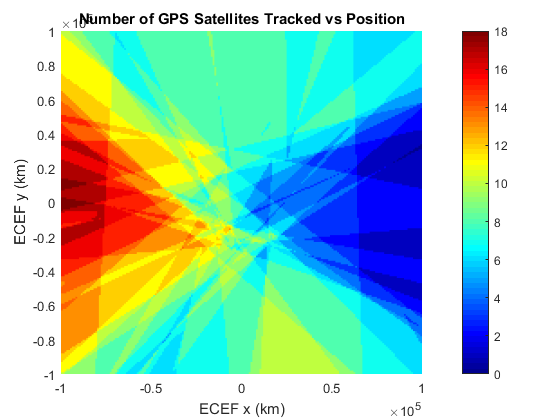
\includegraphics[width=.75\textwidth]{../Images/many.png}
\caption{Tracked Satellites vs Position}
\label{fig:many}
\end{figure}

\FloatBarrier
\subsection{AMSAT OSCAR-40 Replication}
To coarsely verify that the results are sensible, an experiment was set up to replicate the results of AMSAT OSCAR-40's mission. The receiver parameters were set to be equal to those provided by Moreau et al. and placed at an altitude equal to the apogee of the actual AO40 satellite. The number of tracked satellites was calculated every 15 minutes during a simulated 48 hour interval, and the resulting quantity vs time plot is presented below (see Fig. \ref{fig:ao40copy}). Note that, for the majority of the time, no satellites are tracked, with periodic bursts of one or two tracked satellites. This is consistent with the reported findings in \cite{ao40}.

\begin{figure}[h]
\centering
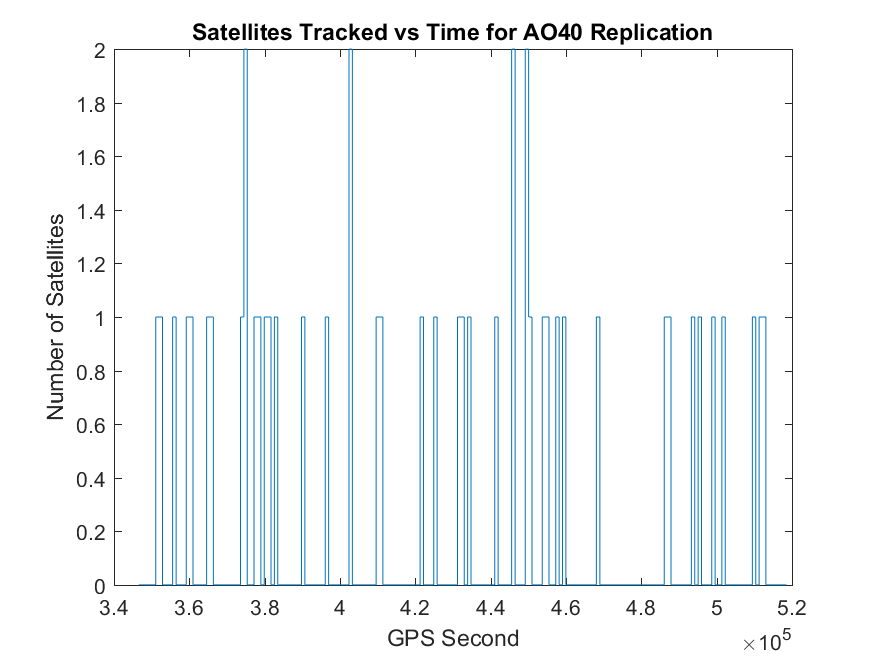
\includegraphics[width=.66\textwidth]{../Images/ao40actual.png}
\caption{Tracked Satellites vs Time}
\label{fig:ao40copy}
\end{figure}

In order to reflect a more modern version of AO40, the tracking threshold was decreased from $40$ dB-Hz to $25$ dB-Hz, while the net gains were assumed to remain the same. The changes reflect an improvement in tracking systems, and a miniaturization of early 2000's components. Figure \ref{fig:ao40new} shows the resulting number of tracked satellites, over the same time period. The drastic increase in number of tracked satellites shows that simply increasing the quality of the tracking  and acquisition system can make the difference between being able to compute a navigational system, and being forced to rely on other external tracking systems. The mean number of satellites tracked is 2.5, compared to the old version's 0.25.

\begin{figure}[h]
\centering
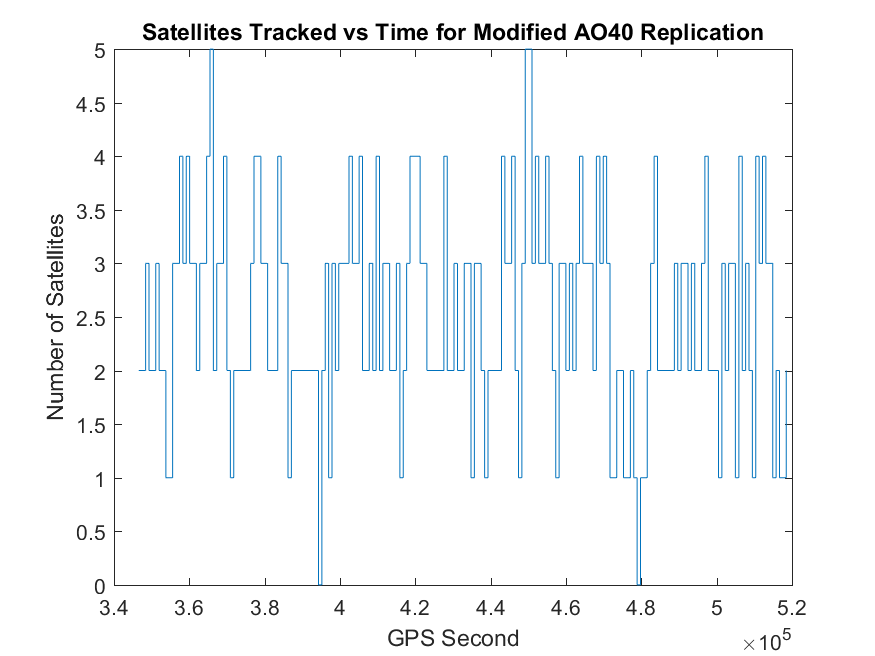
\includegraphics[width=.66\textwidth]{../Images/ao40better.png}
\caption{Tracked Satellites vs Time (Improved System)}
\label{fig:ao40new}
\end{figure}



\FloatBarrier
\section{Conclusions}
GPS provides a system for determining navigational solutions not just on or near Earth's surface, but also at altitudes high above Earth's surface. Modern tracking and acquisition systems allow relatively weak signals to be captured, and it is possible to model the received power of GPS signals at a given location in space. The model relies on GPS gain patterns and attitude models, and varies in time and with receiver parameters. Increasing the receiver sensitivity greatly increases the number of satellites able to be tracked, which intuitively makes sense. A radio telescope pointed at Earth from Pluto would probably be able to determine a navigational solution, its just a matter of high enough gain and low enough noise. More so than providing an upper limit on how high GPS works, this report has illuminated the design considerations that must be accounted for when developing a high altitude GPS receiver.

More work could be done to implement more satellite's gain patterns, rather than just relying on one as a proxy for all of them. Additionally, Lockheed has provided the gain patterns for the signal broadcast at L2 - these could be included to augment the number of observable satellites. In order to actually model what a given satellite would receive, a better model of the receiver is needed. Manufacturer data sheets do not provide a map from reception angles to gain: this would need to be empirically determined. Additionally, testing would reveal better values for other RX parameters.

Finally, there is the potential to somehow incorporate the received signal strength into the measurement model of the navigational solution. This report has defined a model for the $\cnr$ as a function of $r$. By comparing the estimated $\cnr$ to the observed $\cnr$ in terms of the partial derivative, the model could fit into the general navigational solution. For example, if a satellite receives signals from GPS satellites $a$ and $b$ and the receiver knows $r_a$ and $r_b$, then that immediately constrains the possible solution space to those areas in front of satellites $a$ and $b$. 

\pagebreak

\begin{appendices}
\section{Selected Code}
\lstinputlisting[caption={Single Satellite},label={lst:lab1_crs}]{../tests/singlesat.m}
%\pagebreak
\lstinputlisting[caption={Many Satellites},label={lst:lab2_hrs}]{../tests/many.m}
\lstinputlisting[caption={AO-40 Validation},label={lst:lab2_hrs}]{../tests/repeatAO40.m}
\lstinputlisting[caption={Determine Angles},label={lst:lab2_hrs}]{../code/findRotationAngle.m}
\lstinputlisting[caption={Find Sun},label={lst:lab2_hrs}]{../code/findSun.m}
\lstinputlisting[caption={Gain Lookup},label={lst:lab2_hrs}]{../code/SatDirectivityGain.m}
%\pagebreak
\bibliographystyle{ieeetr}
\bibliography{pangea}  
\end{appendices} 

\end{document}
